Za pomoci přístroje Scratch Tester jsme testovali vazbu různých tlustovrstvých past na substrát (Alumina). Přístroj nabízí možnost progresivního testu, při kterém je postupně zvyšována normálová síla (\(F_{Z} \) ). Ve výsledných datech z přístroje jsou k dispozici hodnoty této síly, síly v ose pohybu (\(F_{X} \)) a hodnotu akustické emise smímané mikrofonem, z té by mělo být zjistitelné, jestli došlo k delaminaci vrstvy \cite{DiplomkaScratchTester}. Všechny tyto hodnoty přístroj dává vždy přiřazené ke konkrétní poloze hrotu. 

Testovali jsme tři typy past, získané hodnoty jsou zobrazeny na Obr.~\ref{graf:cermet} (Cermetová pasta), Obr.~\ref{graf:Polymer} (Polymerová pasta) a Obr.~\ref{graf:Rezinat} (Rezinátová pasta).

Následně jsme vytvořenou rýhu analyzovali mikroskopem (TODO). Detail pozorovaných deformací je zobrazen na Obr.~\ref{fig:cer1-jpg} (Cermetová pasta), Obr.~\ref{fig:pol1-jpg} (Polymerová pasta) a Obr.~\ref{fig:rez1-jpg} (Rezinátová pasta).

% Cermet
\begin{figure*}[h!]
    \begin{tikzpicture}
        \centering
        \begin{axis}
            [
            xlabel={ Pozice\ [\unit{\milli\meter}]},
            ylabel={ F \ [\unit{\milli\newton}]},
            axis y line*=left, % dve y osy
            width=1\textwidth,
            height = 0.5\textwidth,
            legend pos=north west
%			xmin=0,
%			ymin=0,
%			xmax=100,
%			ymax=100
            ]
            \addplot[mark=none, mark options={solid}, thick, blue, solid, mark size=3pt] table [skip first n=2, x=A, y=B, col sep=comma] {data/scratchtest/Cermet.csv};
            \addlegendentry{Force Z}

            \addplot[mark=none, mark options={solid}, thick, red, solid, mark size=3pt] table [skip first n=2, x=A, y=D, col sep=comma] {data/scratchtest/Cermet.csv};
            \addlegendentry{Force X}
        \end{axis}   
     
        
%         % Second y axis 
        \begin{axis}
            [
            ylabel={Akustické emise\ [\unit{\decibel}]},
            axis x line=none,
            axis y line*=right,
            width=1\textwidth,
            height = 0.5\textwidth,
            legend pos=north east
%			xmin=0,
%			ymin=0,
%			xmax=100
%			ymax=100
            ]

            \addplot[mark= none, mark options={solid}, thick,  green, dotted, mark size=3pt] table [skip first n=2, x=A, y=C, col sep=comma] {data/scratchtest/Cermet.csv};
            
            \addlegendentry{Akustické emise}
        \end{axis}   
    \end{tikzpicture}
    \caption{Scratch test -- Cermet.}
    \label{graf:cermet}
\end{figure*}

% Polymer
\begin{figure*}[h!]
    \begin{tikzpicture}
        \centering
        \begin{axis}
            [
            xlabel={ Pozice\ [\unit{\milli\meter}]},
            ylabel={ F \ [\unit{\milli\newton}]},
            axis y line*=left, % dve y osy
            width=1\textwidth,
            height = 0.5\textwidth,
            legend pos=north west
%			xmin=0,
%			ymin=0,
%			xmax=100,
%			ymax=100
            ]
            \addplot[mark=none, mark options={solid}, thick, blue, solid, mark size=3pt] table [skip first n=2, x=A, y=B, col sep=comma] {data/scratchtest/Polymer.csv};
            \addlegendentry{Force Z}

            \addplot[mark=none, mark options={solid}, thick, red, solid, mark size=3pt] table [skip first n=2, x=A, y=D, col sep=comma] {data/scratchtest/Polymer.csv};
            \addlegendentry{Force X}
        \end{axis}   
     
        
%         % Second y axis 
        \begin{axis}
            [
            ylabel={Akustické emise\ [\unit{\decibel}]},
            axis x line=none,
            axis y line*=right,
            width=1\textwidth,
            height = 0.5\textwidth,
            legend pos=north east
%			xmin=0,
%			ymin=0,
%			xmax=100
%			ymax=100
            ]

            \addplot[mark= none, mark options={solid}, thick,  green, dotted, mark size=3pt] table [skip first n=2, x=A, y=C, col sep=comma] {data/scratchtest/Polymer.csv};
            
            \addlegendentry{Akustické emise}
        \end{axis}   
    \end{tikzpicture}
    \caption{Scratch test -- Polymer.}
    \label{graf:Polymer}
\end{figure*}

% Rezinat
\begin{figure*}[h!]
    \begin{tikzpicture}
        \centering
        \begin{axis}
            [
            xlabel={ Pozice\ [\unit{\milli\meter}]},
            ylabel={ F \ [\unit{\milli\newton}]},
            axis y line*=left, % dve y osy
            width=1\textwidth,
            height = 0.5\textwidth,
            legend pos=north west
%			xmin=0,
%			ymin=0,
%			xmax=100,
%			ymax=100
            ]
            \addplot[mark=none, mark options={solid}, thick, blue, solid, mark size=3pt] table [skip first n=2, x=A, y=B, col sep=comma] {data/scratchtest/Rezinat.csv};
            \addlegendentry{Force Z}

            \addplot[mark=none, mark options={solid}, thick, red, solid, mark size=3pt] table [skip first n=2, x=A, y=D, col sep=comma] {data/scratchtest/Rezinat.csv};
            \addlegendentry{Force X}
        \end{axis}   
     
        
%         % Second y axis 
        \begin{axis}
            [
            ylabel={Akustické emise\ [\unit{\decibel}]},
            axis x line=none,
            axis y line*=right,
            width=1\textwidth,
            height = 0.5\textwidth,
            legend pos=north east
%			xmin=0,
%			ymin=0,
%			xmax=100
%			ymax=100
            ]

            \addplot[mark= none, mark options={solid}, thick,  green, dotted, mark size=3pt] table [skip first n=2, x=A, y=C, col sep=comma] {data/scratchtest/Rezinat.csv};
            
            \addlegendentry{Akustické emise}
        \end{axis}   
    \end{tikzpicture}
    \caption{Scratch test -- Rezinát.}
    \label{graf:Rezinat}
\end{figure*}


\begin{figure}[h!]
    \centering
    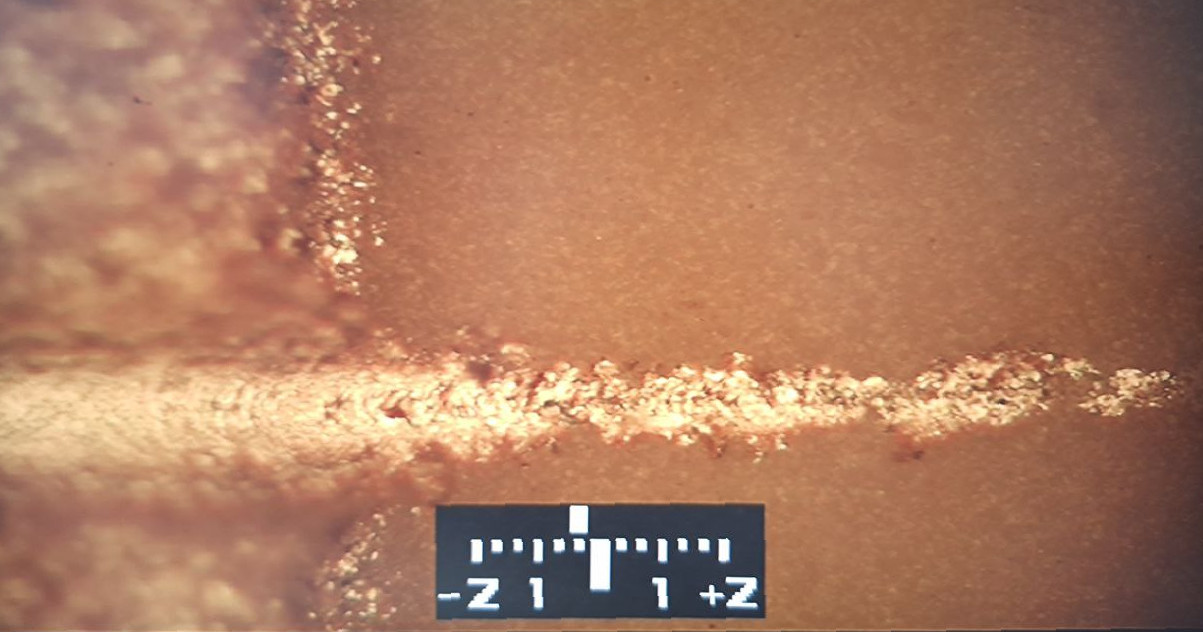
\includegraphics[width=0.8\textwidth]{cer1.jpg}
    \caption{Cermetová pasta po scratch testu (TODO).}
    \label{fig:cer1-jpg}
\end{figure}

\begin{figure}[h!]
    \centering
    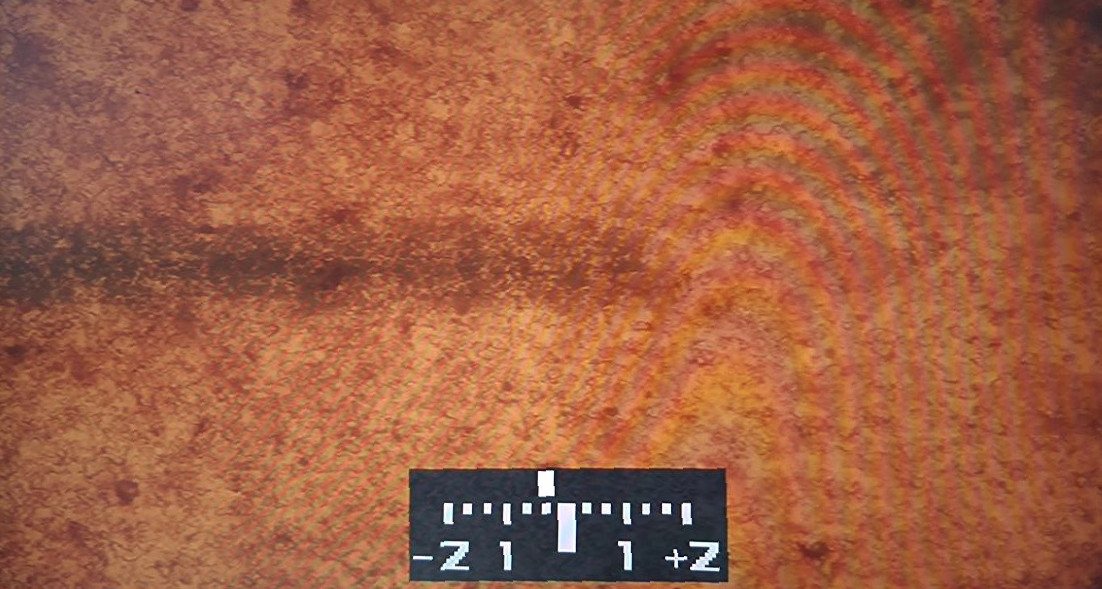
\includegraphics[width=0.8\textwidth]{rez1.jpg}
    \caption{Rezinátová pasta po scratch testu (TODO).}
    \label{fig:rez1-jpg}
\end{figure}

\begin{figure}[h!]
    \centering
    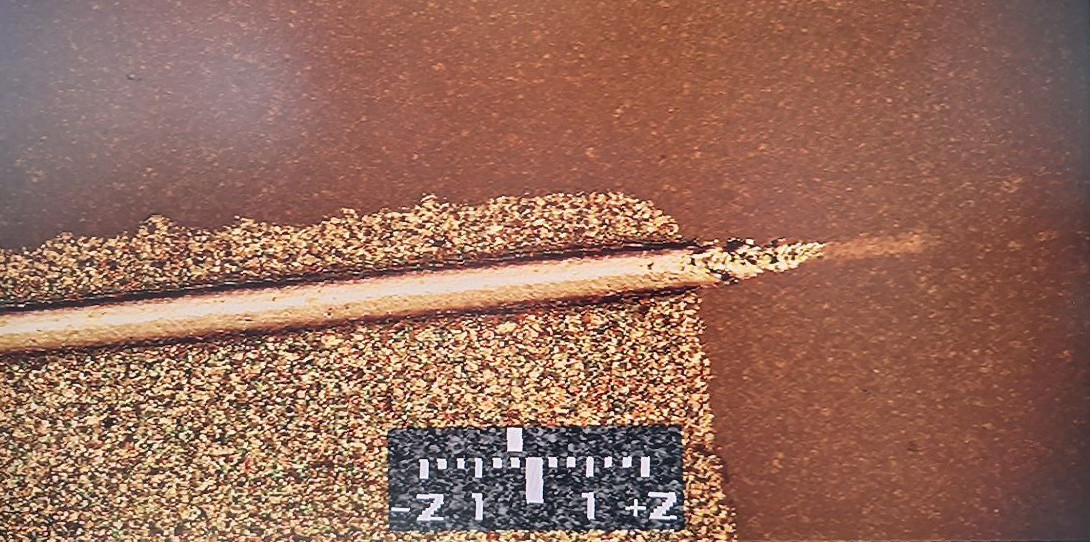
\includegraphics[width=0.8\textwidth]{pol1.jpg}
    \caption{Polymerová pasta po scratch testu (TODO).}
    \label{fig:pol1-jpg}
\end{figure}
